\section{Phase 1}
% Description of your dataset goes here.
\subsection{Data Cleaning}

\subsubsection{Raw data overview}
This chart contains the percentage of non-applicable (N/A) data and the uniqueness of each original feature. During the forthcoming stages of analysis and data cleansing, certain unique identifiers, such as \texttt{app\_id}, might be discarded due to their limited informative value. \texttt{minimum\_installs} and \texttt{maximum\_installs} represent two distinct aspects of installation counts: the former indicates a range, whereas the latter provides a precise, continuous figure. In subsequent steps, I will conduct a series of operations to evaluate the relevance of each feature, making essential modifications to optimize the data for the training process.

\begin{figure}[h]
\centering
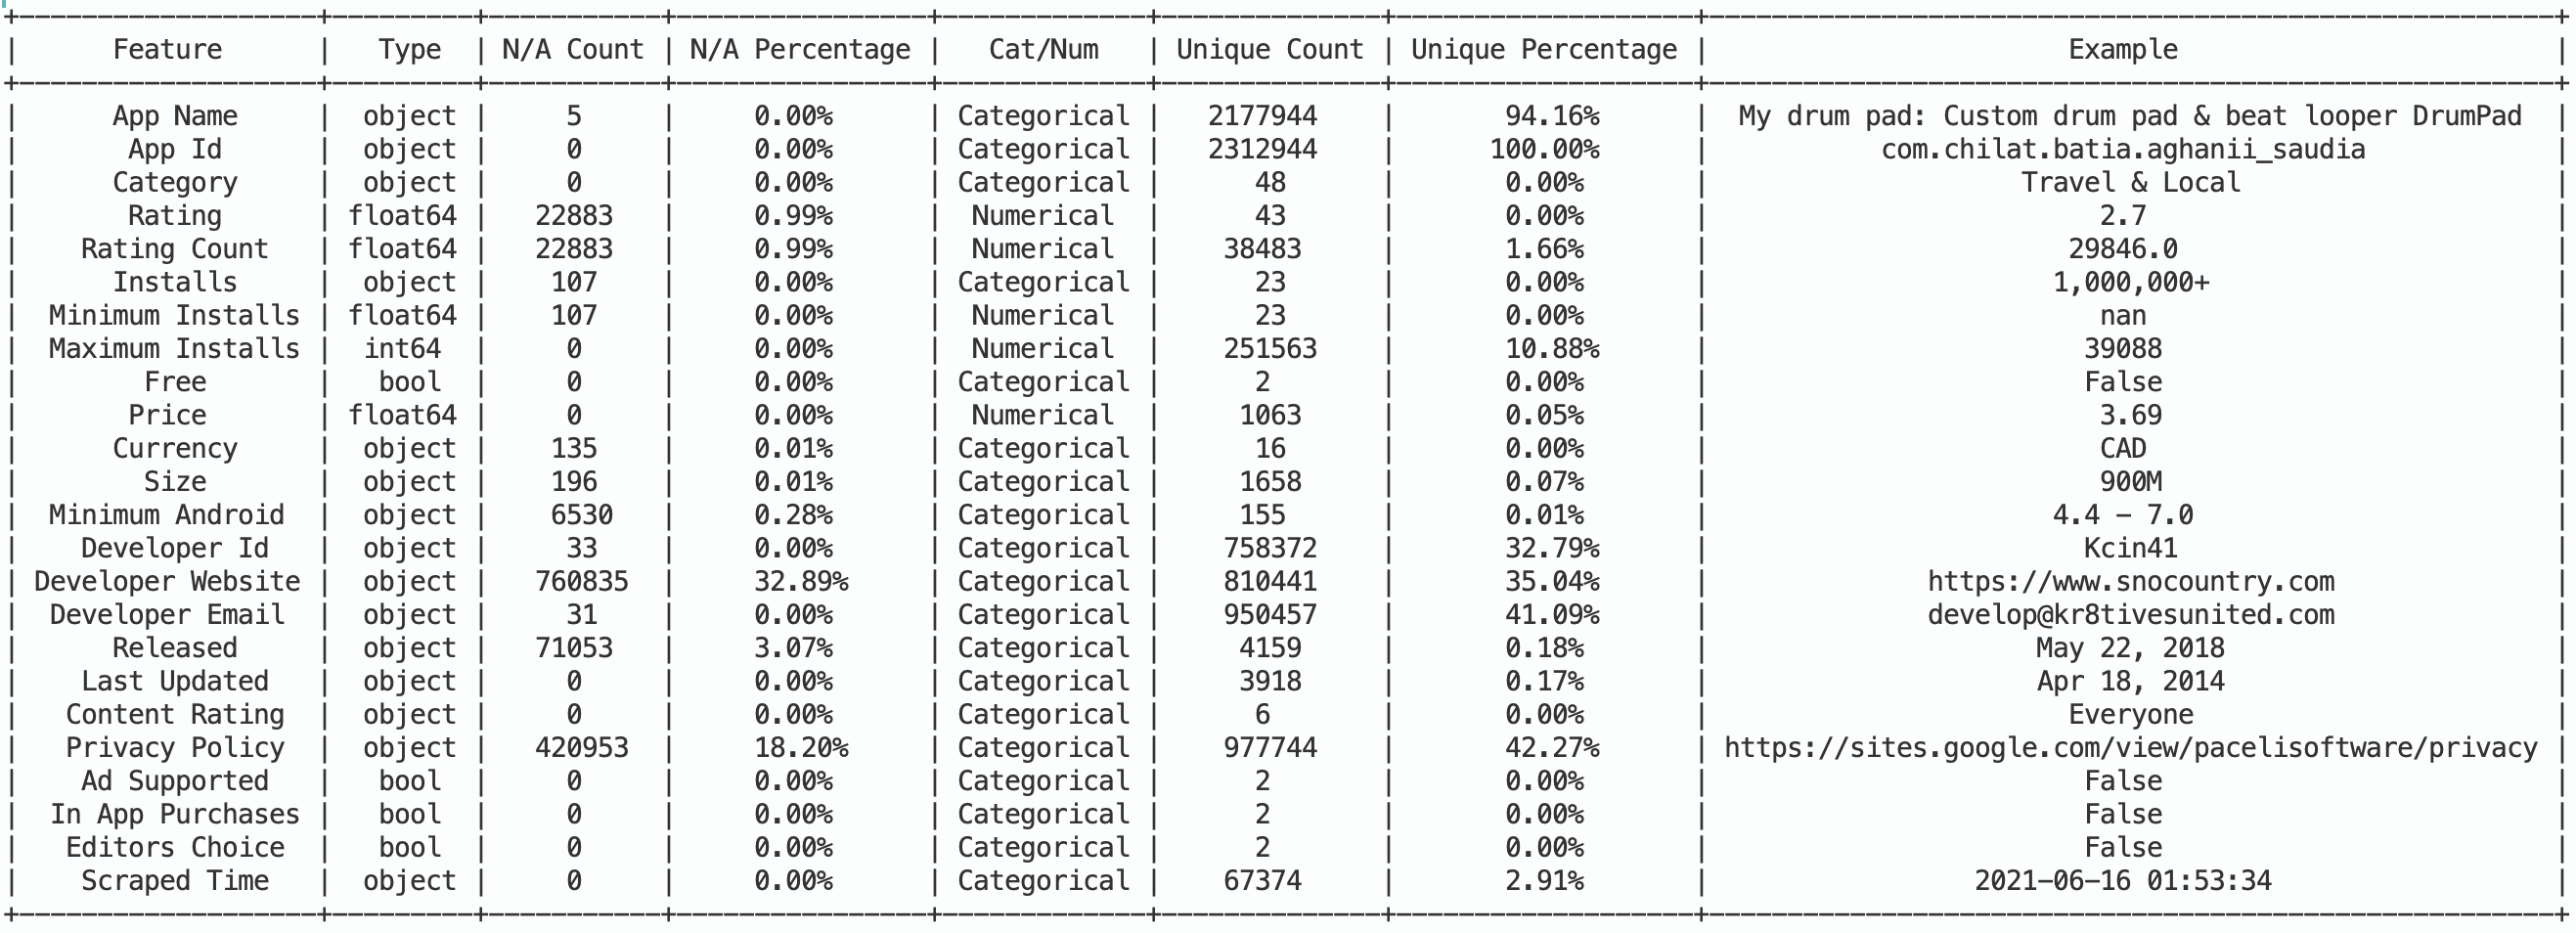
\includegraphics[width=0.8\textwidth]{docs//assets/raw-data-overview.png}
\caption{Raw data overview}
\end{figure}

\subsubsection{N/A values percentage}
% Indentation for this section
For Developer Website and Privacy Policy, due to high observation of N/A values, removing the features makes more sense than removing rows with N/A values.

\subsection{Data Duplication}

\subsubsection{Duplication in Currency column}
% Indentation for this section
\begin{figure}[h]
\centering
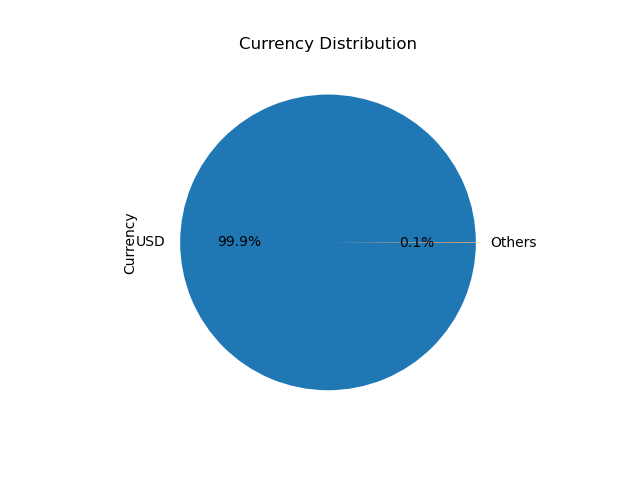
\includegraphics[width=0.8\textwidth]{docs//assets/currency.png}
\caption{Currency Distribution}
\end{figure}
In Figure X, it is evident that the USD currency represents over 99.9\% of the dataset. By removing observations in other currencies and subsequently deleting the Currency column, we can retain 99.9\% of the data while effectively reducing its dimensionality. This approach streamlines the dataset, focusing on the predominant currency for a more efficient analysis.

\subsubsection{Duplication between Installs and Minimum Installs}
% Indentation for this section
The dataset contains three columns related to app installations, each named with variations of the word Installs. Upon examination, \texttt{maximum\_installs} is found to be a continuous numerical value, whereas Installs and \texttt{minimum\_installs} represent a range, indicating the number of app downloads. Additionally, the Installs column includes characters such as \texttt{+} and \texttt{,}. These issues are now fixed.

\subsubsection{Duplication between Free and Price}
% Indentation for this section
Given that the price of free items is listed as 0, the Free column becomes redundant and has therefore been removed from the dataset.

\subsection{Aggregation}
% Indentation for the section content
\subsubsection{Aggregation of Android versions}
% Indentation for this section
The \texttt{minimum\_android} column comprises 27 unique values, each representing a different Android version required for the app's operation. These versions are strings that are not likely to be encoded, such as \texttt{4.1.2}. Given that variations in minor versions do not significantly enhance the analysis of this dataset, a more effective approach is to aggregate these versions by their major numbers (e.g., 4, 5, etc.).

\subsection{Down Sampling}
% Indentation for the section content
\subsubsection{Slicing the dataset}
% Indentation for this section
The dataset has a wide range of data distribution. Install count that is extremely low or high is not the main focus of this analysis. As a result, a slice of data that \texttt{installCount} is between 100k and 10M is extracted for analysis.

\subsection{Dimensionality Reduction}
\subsubsection{Random Forest Analysis}
% Indentation for this section
% \textbf{Steps:}
% \begin{enumerate}
%     \item \textbf{Data Preparation}
%     \begin{itemize}
%         \item Remove target variables
%         \item Convert categorical columns into dummy variables using \texttt{pd.get\_dummies}
%     \end{itemize}
%     \item \textbf{Split the data}
%     \item \textbf{Model initialization and training}
%     \item \textbf{Model prediction}
%     \item \textbf{Feature importance visualization}
% \end{enumerate}
\begin{figure}[h]
\centering
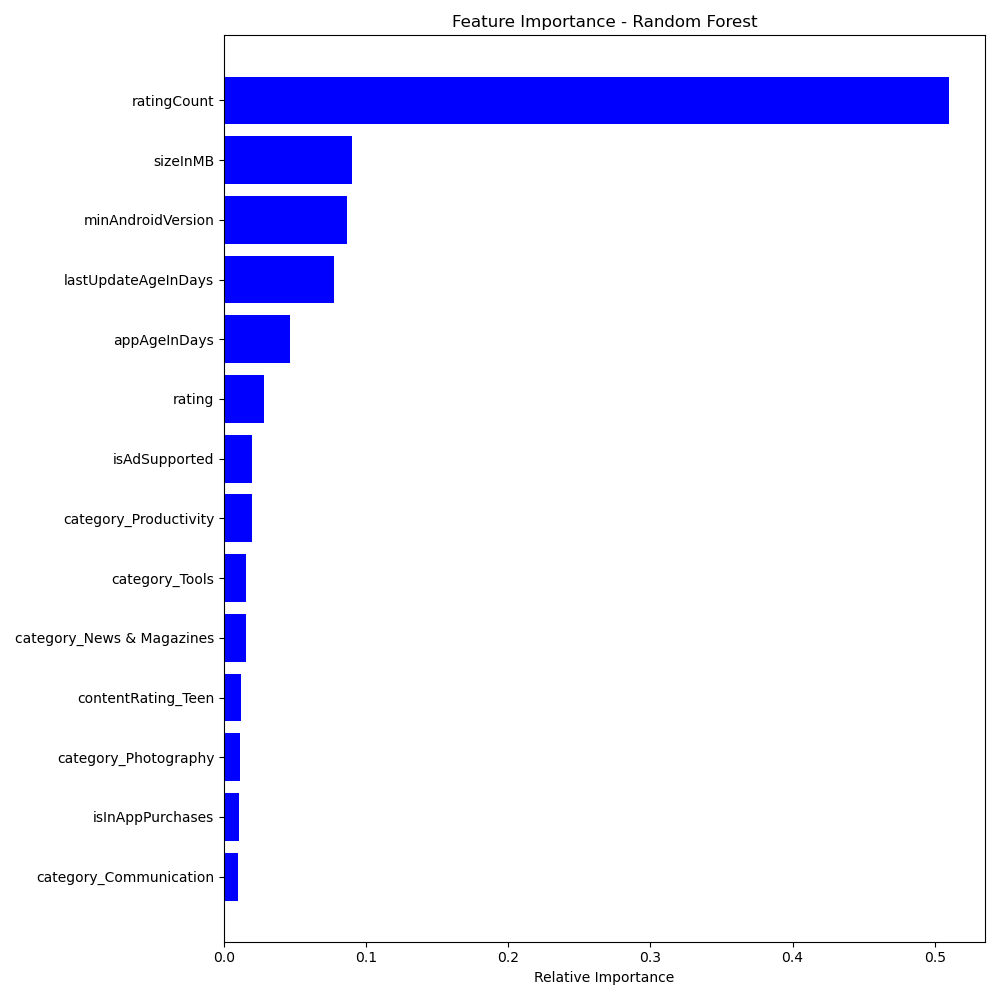
\includegraphics[width=\textwidth]{docs//assets/rfa.png}
\caption{Feature Importance - Random Forest Analysis}
\end{figure}
% Indentation for this section
The horizontal bar plot in Figure X allows us to infer that \texttt{rating\_count} is the most significant feature, followed by \texttt{size\_in\_mb}, \texttt{min\_android\_version}, \texttt{last\_update\_age\_in\_days}, and \texttt{app\_age\_in\_days}. This insight, derived from the Random Forest Analysis, guides subsequent preprocessing steps, aiding in decisions regarding the inclusion or exclusion of specific features.

\subsubsection{Principle Component Analysis and Condition Number}
% Indentation for this section
Figure X demonstrates that a combination of 10 features cumulatively accounts for 85\% of the variance. The dataset, transformed through PCA, consists of 68 columns, reduced from the original 71. This reduction is likely due to the application of \texttt{pd.get\_dummies} on three features, suggesting that PCA has effectively discarded three columns whose information is captured by the remaining data.

\begin{figure}[h]
\centering
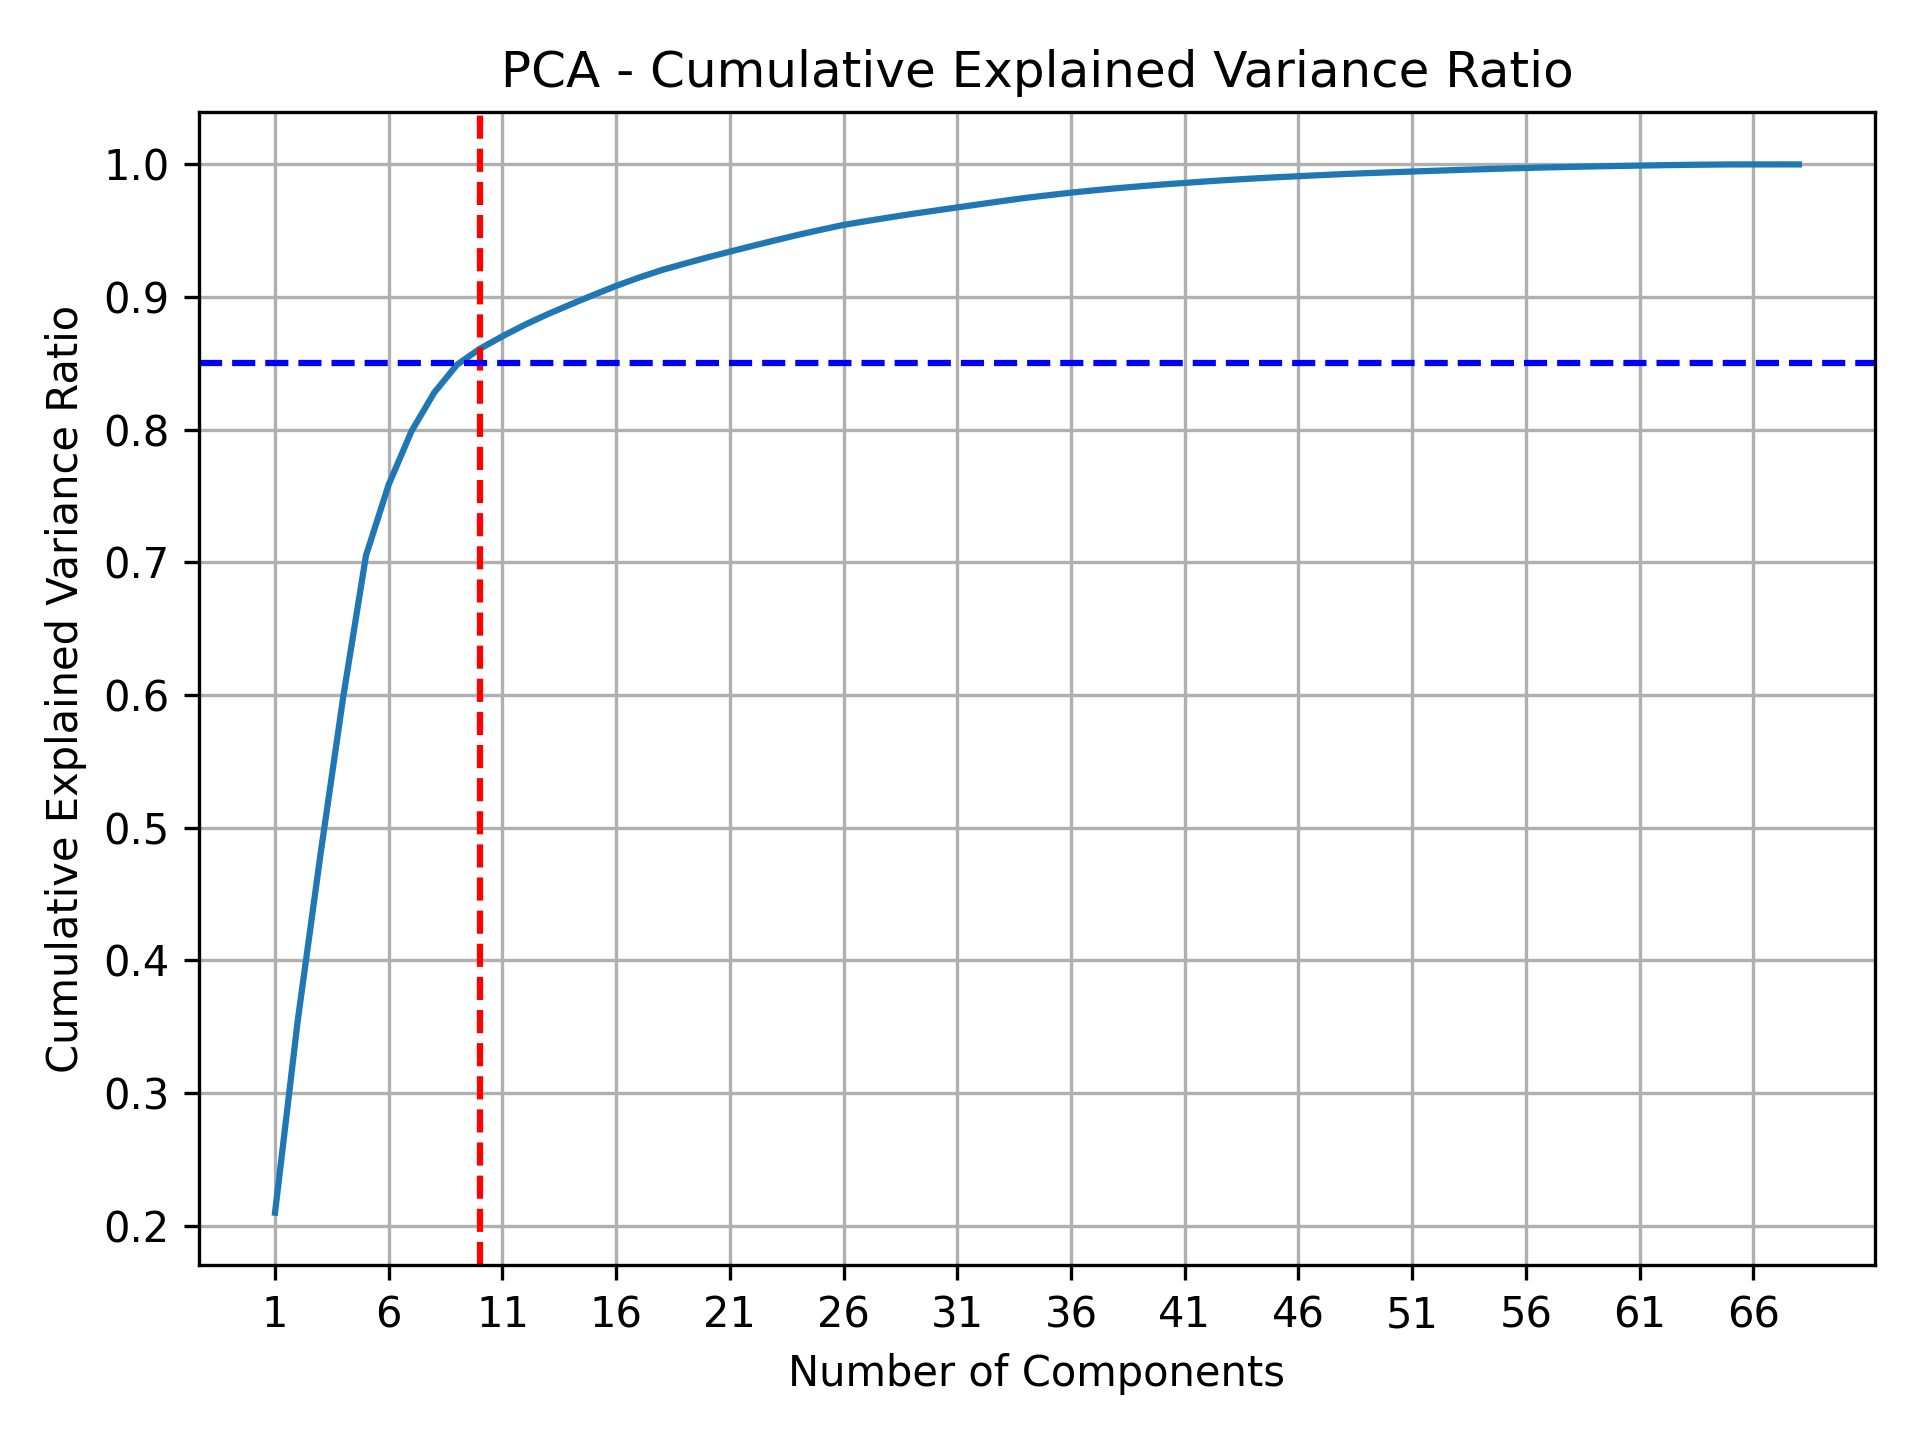
\includegraphics[width=\textwidth]{docs//assets/pca.png}
\caption{Explained Variance Ratio - PCA}
\end{figure}

The program additionally computed the condition number. Prior to the PCA transformation, the condition number was exceedingly high. However, following the transformation, it significantly reduced to 164.65. This decrease in the condition number implies that potential collinearity has been eliminated. Such collinearity might have originated from the use of the \texttt{get\_dummies} method.



\begin{center}
Comparison of Condition Number
\end{center}

% \begin{tabular}{rr}
% \toprule
% \midrule
% Original condition number & PCA transformed condition number & \
% \midrule
% 75869592332155.22 & 164.65 & \
% \bottomrule
% \end{tabular}

\subsubsection{Singular Value Decomposition Analysis}

\begin{figure}[h]
\centering
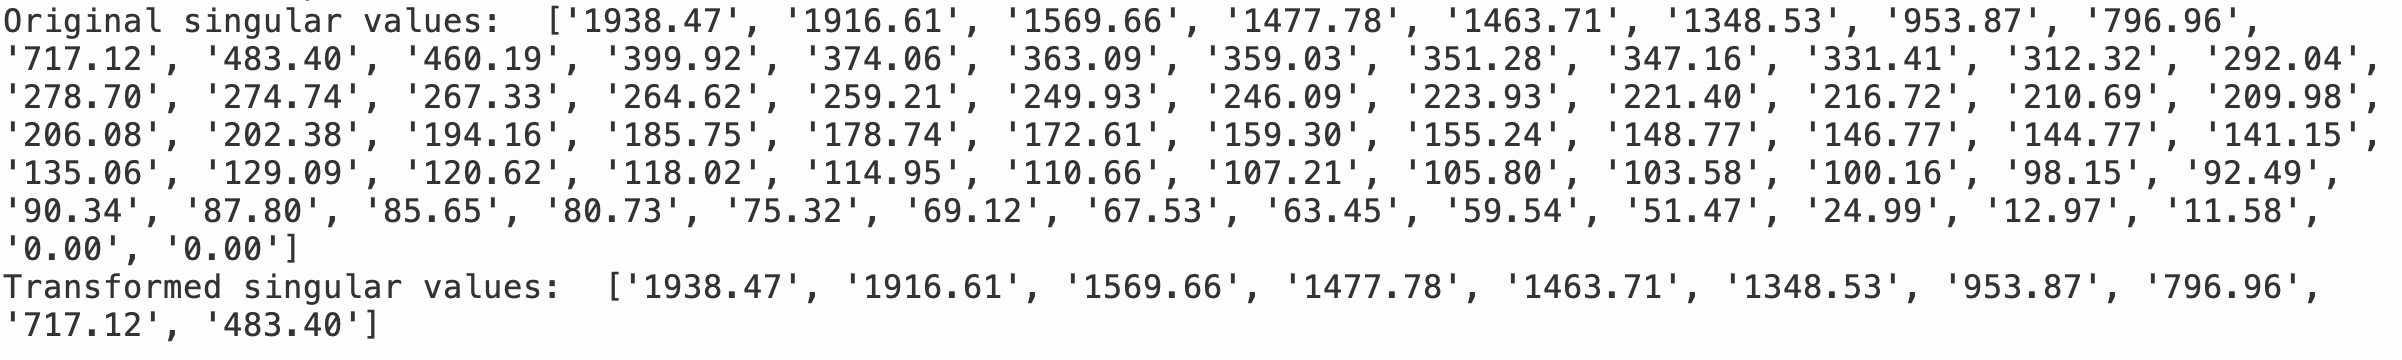
\includegraphics[width=\textwidth]{docs//assets/svd.png}
\caption{Singular Values of Data}
\end{figure}

Following the PCA analysis, 10 features were chosen for the SVD transformation. Figure X presents a comparison of the dataset's singular values before and after the SVD transformation. It is observed that the singular values remain consistent throughout the process. The transformed dataset comprises 10 singular values, each representing the most variance in the data.

\subsubsection{Variance Inflation Factor (VIF) Analysis}

\begin{figure}[h]
\centering
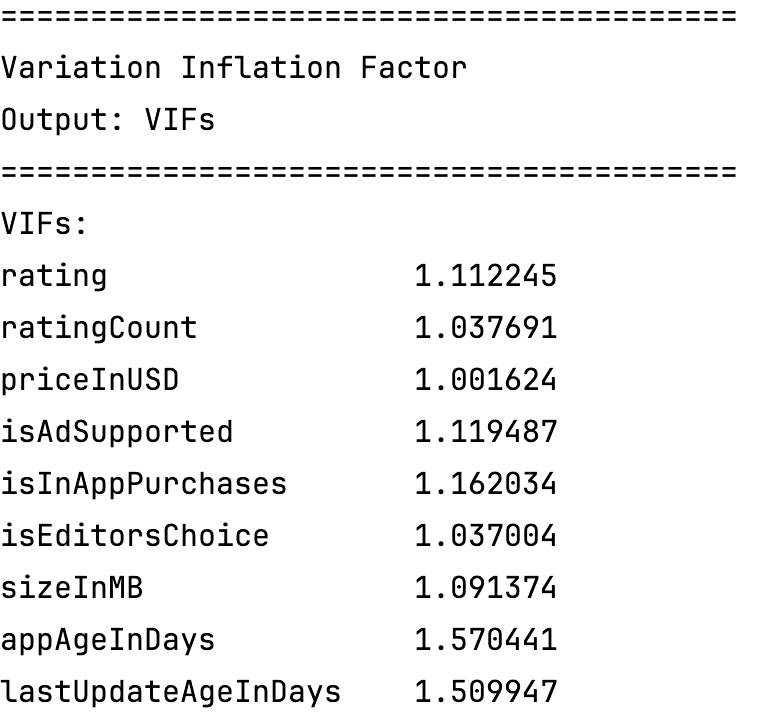
\includegraphics[width=0.5\textwidth]{docs//assets/vif.png}
\caption{VIF of Features}
\end{figure}

Figure X displays the VIF for each numeric feature in the dataset. All VIF values are below 2.5, indicating an absence of collinearity within this dataset. As per various sources, a VIF greater than 5 is generally considered a cause for concern regarding collinearity.

\subsubsection{Collinearity Analysis}

The VIF analysis clearly indicates the absence of collinearity in this dataset. However, the application of one-hot encoding to categorical features did introduce some degree of collinearity, as revealed by the PCA. This issue can be addressed by dropping one column from each set of dummy variables.

\subsubsection{Observation on Dimensionality Reduction}

Comparing the methods used, Random Forest Analysis is notably informative, providing valuable insights into feature importance, an aspect not directly addressed by PCA. SVD could be advantageous for datasets with images and videos, aiding in data compression and meaningful information extraction, though its effectiveness varies. In this dataset, the impact of SVD is less distinct due to the addition of 62 dummy variables through one-hot encoding, which are less amenable to decomposition and may contribute to multicollinearity. VIF analysis, on the other hand, is extremely useful as it precisely quantifies dataset collinearity.

Despite a longer computation time, Random Forest Analysis is recommended for this dataset as a better approach for feature selection rather than traditional dimensionality reduction. It provides essential information on each feature, which is highly beneficial for informed decision-making in feature selection.

\subsection{Discretization \& Binarization}
\subsubsection{Discretization of \texttt{minimumInstalls} Column}

The Google Play Store categorizes app installations into 18 distinct groups, ranging from 0, 1, 5, 10, 50, 100, up to 5B and 10B. Utilizing this categorical feature as a target in analysis can lead to excessive complexity and a heightened risk of overfitting due to the multitude of classes. To mitigate this issue, regrouping the installation categories proves to be a viable solution. Figure X illustrates the distribution of values in the \texttt{installRange} after this modification. The data has been reorganized into five new, balanced groups.

\subsection{One-hot Encoding of Categorical Values}

By applying \texttt{pd.get\_dummies} to the \texttt{category}, \texttt{minAndroidVersion}, and \texttt{contentRating} columns, these categorical variables are transformed into a numerical format suitable for analysis. According to the Random Forest Analysis, the most significant features include \texttt{category\_Productivity}, \texttt{category\_Social}, \texttt{minAndroidVersion\_8}, and \texttt{minAndroidVersion\_7}. Based on the combined insights from Random Forest and PCA, these selected columns are deemed crucial as they are among the top contributors to explaining at least 85\% of the dataset's variance.

\subsection{Variable Transformation}

Standardization is not necessary for decision tree and several other algorithms due to their insensitivity to data scale. In this part of the project, a new standardized dataframe is created, ensuring that the original data remains unaltered. This approach allows for the flexibility to apply different algorithms, both those that benefit from standardization and those that do not.

\subsection{Anomaly Detection}

\begin{figure}[h]
\centering
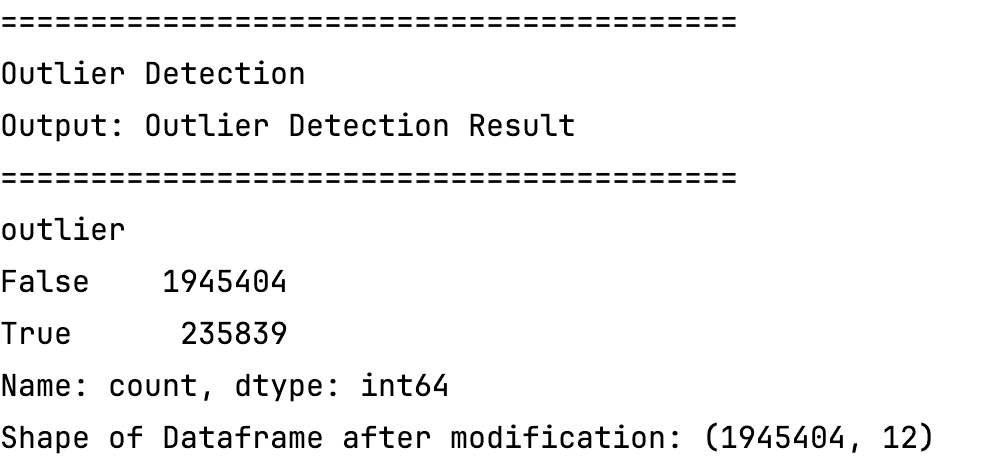
\includegraphics[width=0.5\textwidth]{docs//assets/outlier.png}
\caption{Outlier Detection Console Message}
\end{figure}

In this part of the pre-processing, normalization tests and IQR outlier removal are utilized. The target observes no distribution at first, this issue is solved by applying \texttt{np.log10}. Unfortunately even after logarithmic transformation, the data did not pass \textbf{Shapiro test}. Figure X shows the Q-Q plot of Install vs. Normal Distribution. 

After outlier removal using IQR method, the target still can not pass Shapiro test. In order to keep useful information, no further outlier removal is executed.

% In this analysis, the Mahalanobis distance, in conjunction with the chi-squared distribution, is utilized to identify outliers in the dataset. It's important to note that the squared Mahalanobis Distance adheres to a Chi-Square distribution. The degrees of freedom for the chi-squared test are set at 11, accounting for 10 variables and one target in the dataset. A significance level of 0.1 is chosen for outlier detection, which is a common practice in statistical analysis to balance between sensitivity and specificity in identifying outliers. Consequently, this approach led to the identification and proposed removal of approximately 235,840 observations, equating to roughly 10.8\% of the data, as outliers.

\subsection{Sample Covariance Matrix and Sample Pearson Correlation Coefficient Matrix}

\begin{figure}[h]
\centering
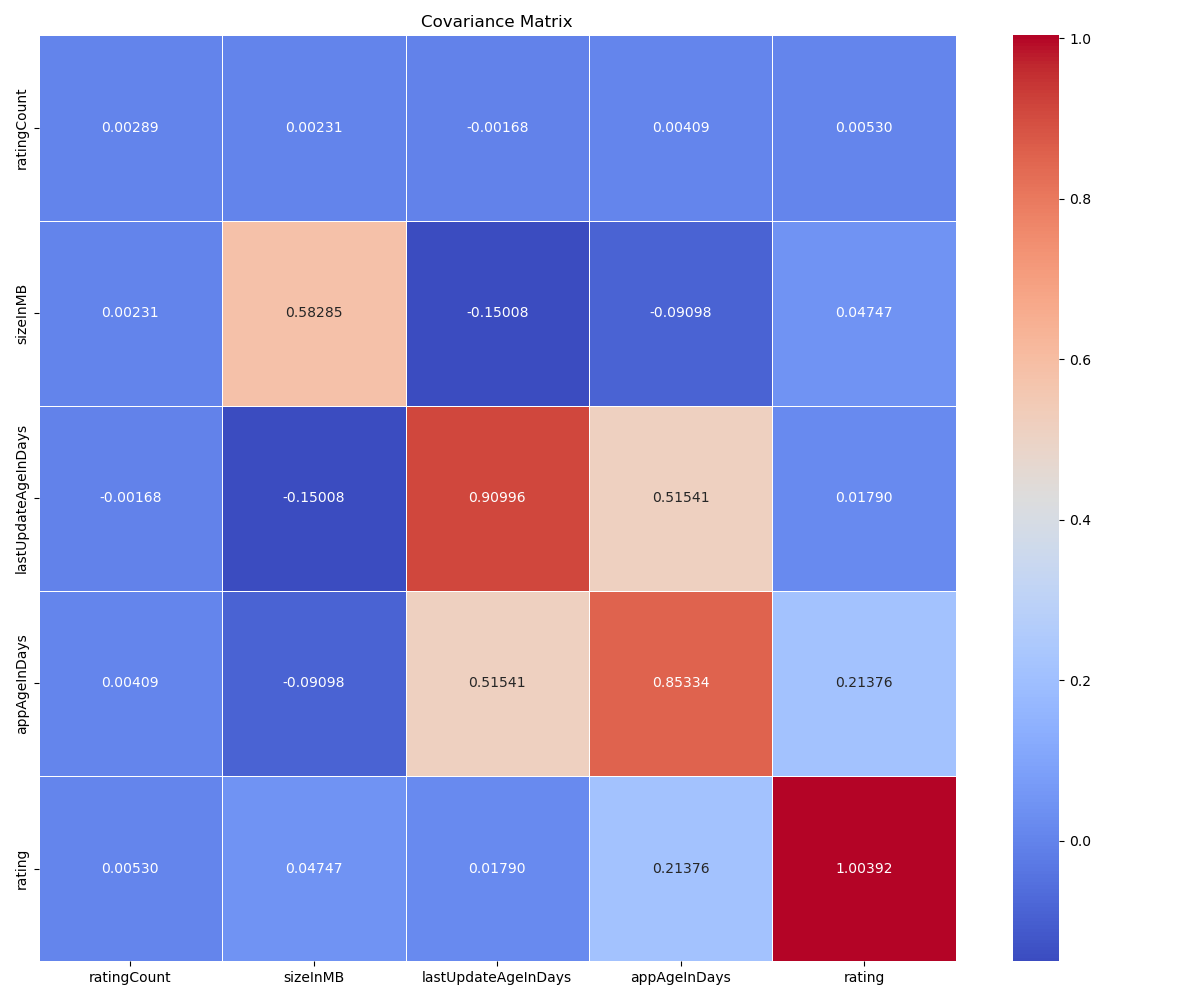
\includegraphics[width=\textwidth]{docs//assets/cov.png}
\caption{Sample Covariance Matrix}
\end{figure}

\begin{figure}[h]
\centering
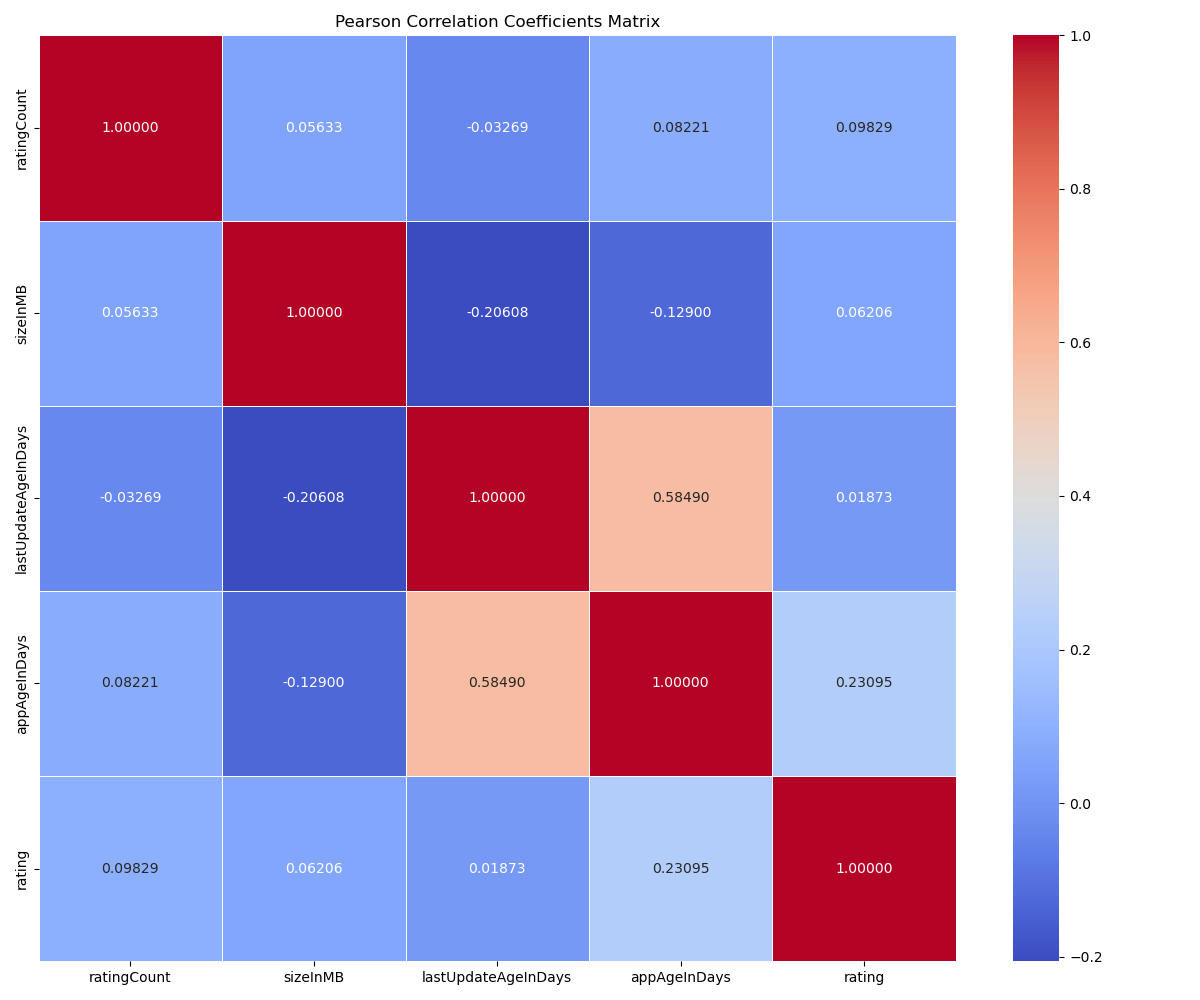
\includegraphics[width=\textwidth]{docs//assets/cor.png}
\caption{Sample Pearson Covariance Correlation Matrix}
\end{figure}

Figure X and Figure Y represent the covariance matrix and the correlation matrix of the dataset, respectively. The low covariance, combined with the earlier analysis indicating a lack of collinearity among variables, is beneficial for model training. This absence of collinearity, particularly in regression models, reduces the risk of multicollinearity, leading to more stable estimates of regression coefficients

\subsection{Balanced or Imbalanced Data}

\begin{figure}[h]
\centering
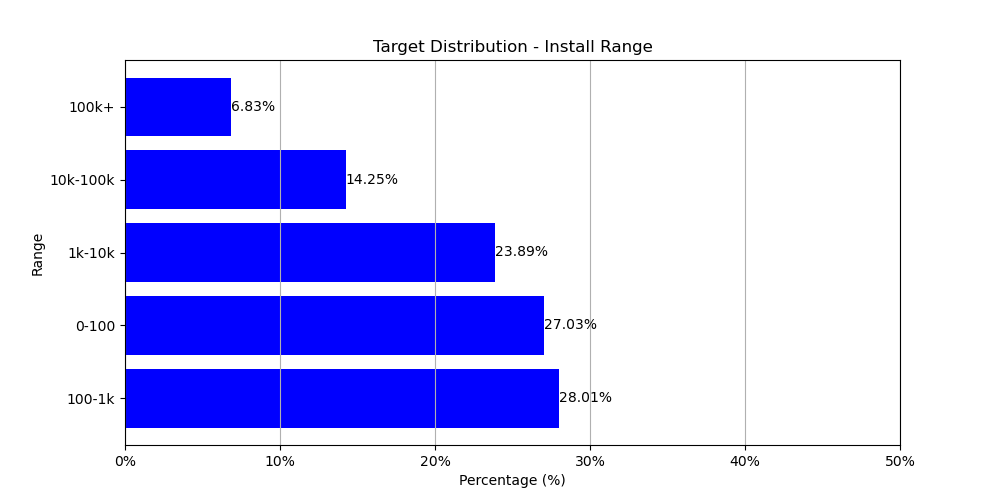
\includegraphics[width=\textwidth]{docs//assets/target.png}
\caption{Distribution of Target values}
\end{figure}

The current distribution of targets depicted in Figure X indicates a imbalanced composition, with no single group dominating the target dataset.

In order to make sure target is balanced, \texttt{pd.qcut} is utilized. Figure X shows the balanced target distribution after discretization and binarization.

% Rest of the document continues with similar formatting and structuring...


% \section{Phase 1}
% % Description of your dataset goes here.
% \subsection{Data Cleaning}

% \subsubsection{Raw data overview}
% This chart contains the percentage of non-applicable (N/A) data and the uniqueness of each original feature. During the forthcoming stages of analysis and data cleansing, certain unique identifiers, such as App Id, might be discarded due to their limited informative value. 'Minimum Installs' and 'Maximum Installs' represent two distinct aspects of installation counts: the former indicates a range, whereas the latter provides a precise, continuous figure. In subsequent steps, I will conduct a series of operations to evaluate the relevance of each feature, making essential modifications to optimize the data for the training process.

% \begin{figure}[h]
% \centering
% 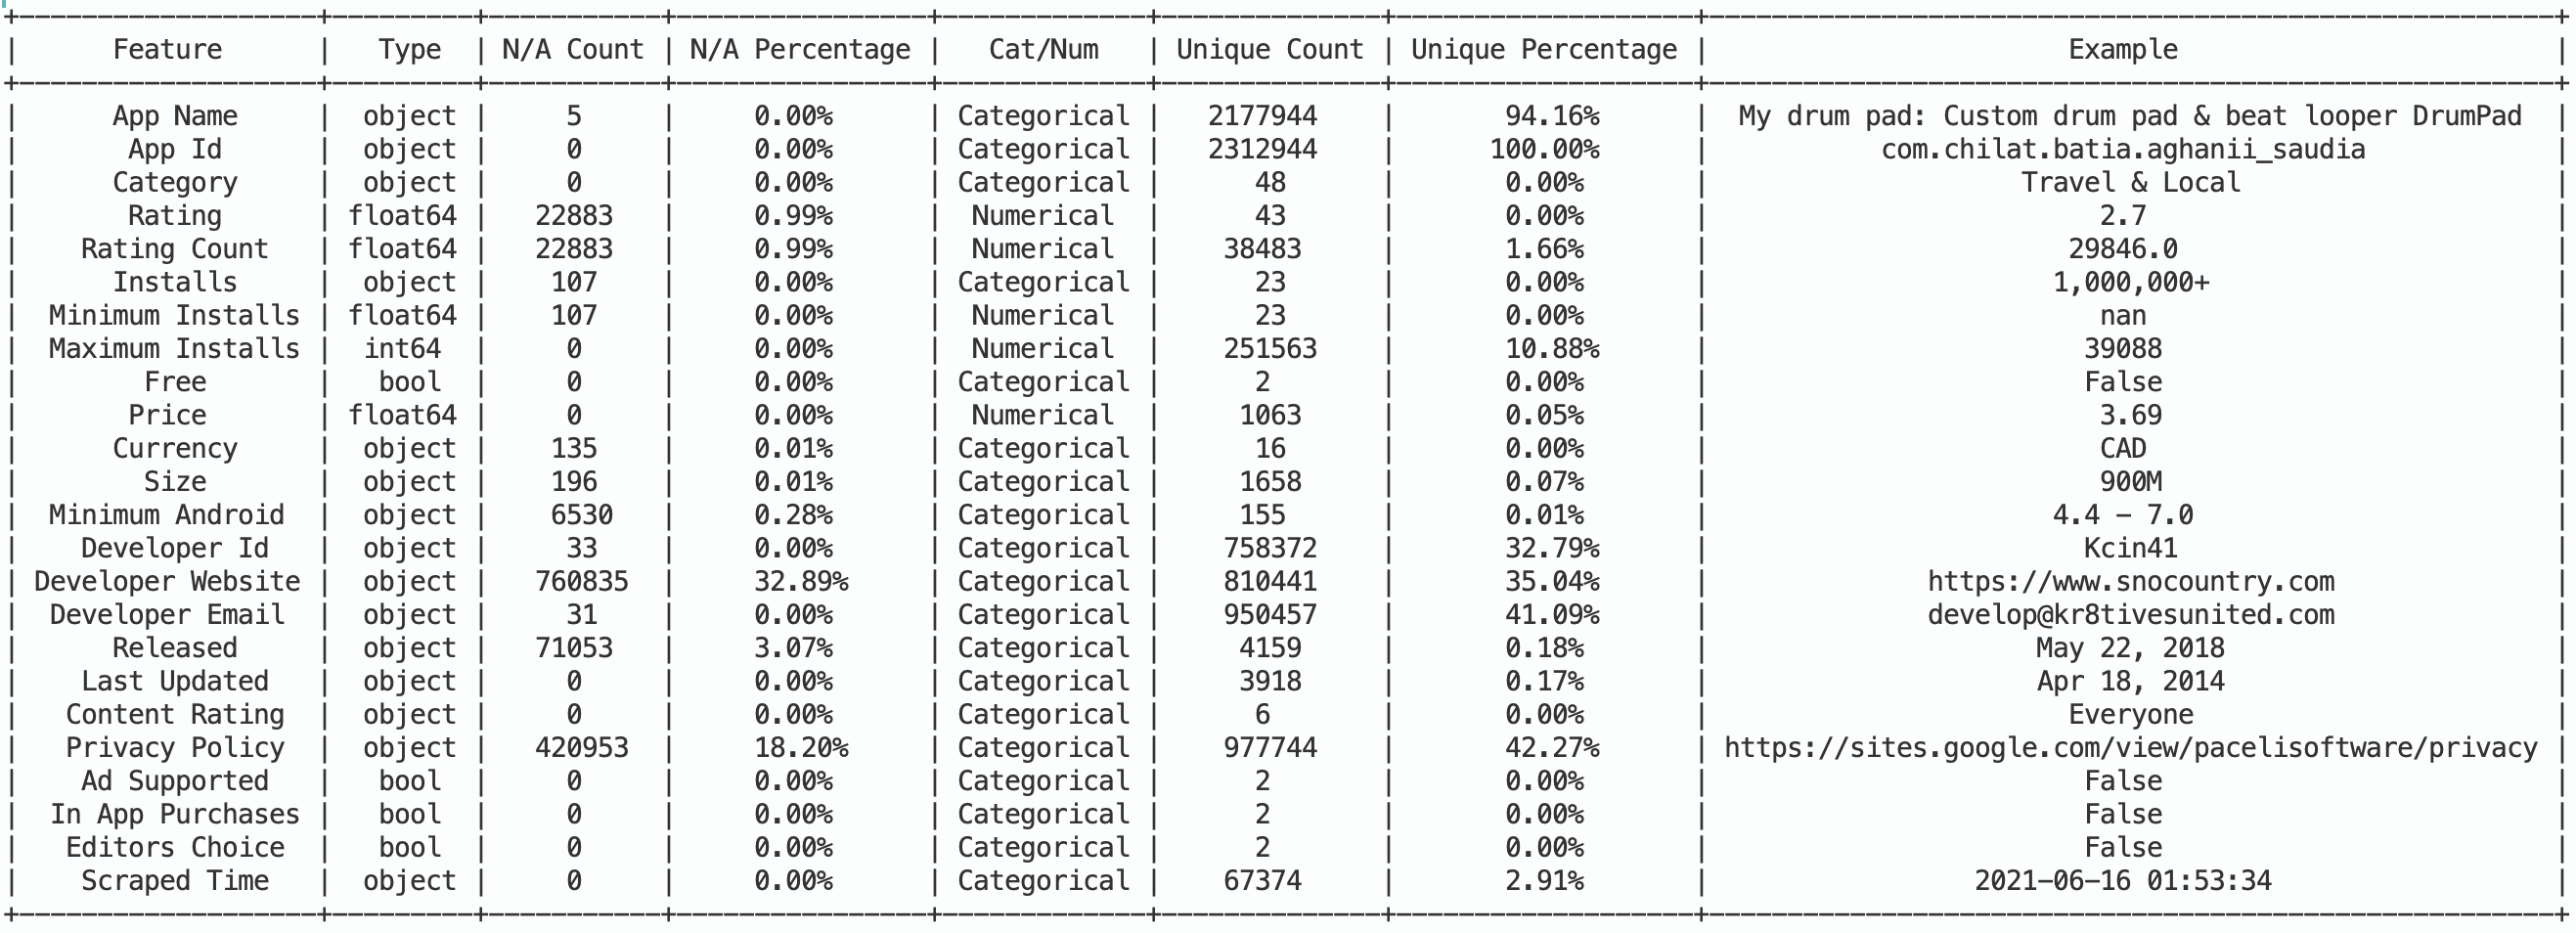
\includegraphics[width=0.8\textwidth]{docs//assets/raw-data-overview.png}
% \caption{Raw data overview}
% \end{figure}

% \subsubsection{N/A values percentage}

% \begin{figure}[h]
% \centering
% 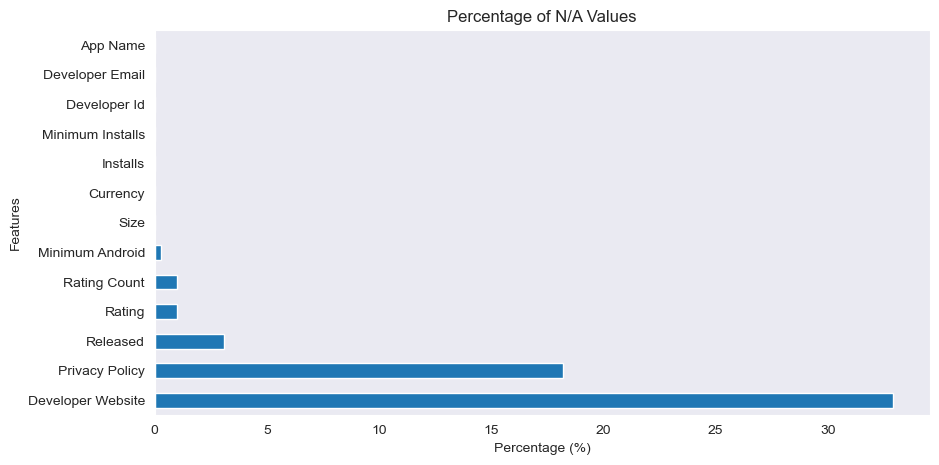
\includegraphics[width=1\textwidth]{docs//assets/percentage_na.png}
% \caption{N/A values percentage}
% \end{figure}

% For Developer Website and Privacy Policy, due to high observation of N/A values, removing the features makes more sense than removing rows with N/A values.

% \subsection{Data Duplication}

% \subsubsection{Duplication in "Currency" column}

% \begin{figure}[h]
% \centering
% 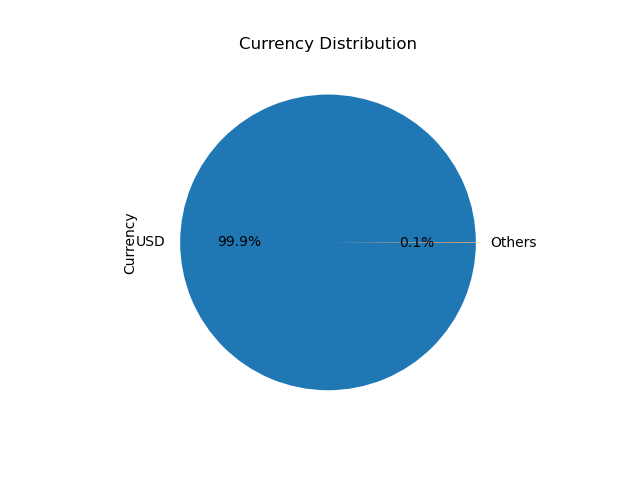
\includegraphics[width=\textwidth]{docs//assets/currency.png}
% \caption{Currency Distribution}
% \end{figure}

% In Figure X, it is evident that the "USD" currency represents over 99.9\% of the dataset. By removing observations in other currencies and subsequently deleting the "Currency" column, we can retain 99.9\% of the data while effectively reducing its dimensionality. This approach streamlines the dataset, focusing on the predominant currency for a more efficient analysis.

% \subsubsection{Duplication between "Installs" and "Minimum Installs"}

% \begin{figure}[h]
% \centering
% \includegraphics[width=\textwidth]{docs//assets/pic.png}
% \caption{Currency Distribution}
% \end{figure}

% The dataset contains three columns related to app installations, each named with variations of the word 'Installs.' Upon examination, 'Maximum Installs' is found to be a continuous numerical value, whereas 'Installs' and 'Minimum Installs' represent a range, indicating the number of app downloads. Additionally, the 'Installs' column includes characters such as '+' and ',', categorizing it as a string. The code presented in Figure X is used to determine whether the 'Installs' and 'Minimum Installs' columns are equivalent.

% \subsubsection{Duplication between "Free" and "Price"}

% Given that the price of free items is listed as 0, the 'Free' column becomes redundant and has therefore been removed from the dataset.


% \subsection{Aggregation}

% \subsubsection{Aggregation of Android versions}

% \begin{figure}[h]
% \centering
% \includegraphics[width=\textwidth]{docs//assets/pic.png}
% \caption{Currency Distribution}
% \end{figure}

% \text{The 'Minimum Android' column comprises 27 unique values, each representing a different Android version required for the app's operation. These versions are denoted as strings, such as '4.1.2'. Given that variations in minor versions do not significantly enhance the analysis of this dataset, a more effective approach involves aggregating these versions by their major numbers (e.g., 4, 5, etc.). Figure X displays a pie chart illustrating the distribution of these major Android versions after aggregation.}

% \subsection{Dimensionality Reduction}
% \subsubsection{Random Forest Analysis}
% \textbf{Steps:}
% \begin{enumerate}
%     \item \textbf{Data Preparation}
%     \begin{itemize}
%         \item Remove target variables
%         \item Convert categorical columns (category, contentRating) into dummy variables using \texttt{pd.get\_dummies}
%     \end{itemize}
%     \item \textbf{Split the data}
%     \item \textbf{Model initialization and training}
%     \item \textbf{Model prediction}
%     \item \textbf{Feature importance visualization}
% \end{enumerate} % End the enumerate environment here
% \begin{figure}[h]
% \centering
% \includegraphics[width=\textwidth]{docs//assets/pic.png}
% \caption{Currency Distribution}
% \end{figure}
% % Now the text is no longer part of the enumerate environment
% \noindent\text{The horizontal bar plot in Figure X allows us to infer that 'ratingCount' is the most significant feature, followed by 'sizeInMB', 'minAndroidVersion', 'lastUpdateAgeInDays', and 'appAgeInDays'. This insight, derived from the Random Forest Analysis, guides subsequent preprocessing steps, aiding in decisions regarding the inclusion or exclusion of specific features.}

% \subsubsection{Principle Component Analysis and Condition Number}

% \noindent\text{Figure X demonstrates that a combination of 10 features cumulatively accounts for 85\% of the variance. The dataset, transformed through PCA, consists of 68 columns, reduced from the original 71. This reduction is likely due to the application of pd.get\_dummies on three features, suggesting that PCA has effectively discarded three columns whose information is captured by the remaining data.}

% \begin{figure}[h]
% \centering
% \includegraphics[width=\textwidth]{docs//assets/pic.png}
% \caption{Currency Distribution}
% \end{figure}

% \text{The program additionally computed the condition number. Prior to the PCA transformation, the condition number was exceedingly high. However, following the transformation, it significantly reduced to 164.65. This decrease in the condition number implies that potential collinearity has been eliminated. Such collinearity might have originated from the use of the get\_dummies method.}

% \begin{figure}[h]
% \centering
% \includegraphics[width=\textwidth]{docs//assets/pic.png}
% \caption{Currency Distribution}
% \end{figure}

% \subsubsection{Singular Value Decomposition Analysis}

% \begin{figure}[h]
% \centering
% \includegraphics[width=\textwidth]{docs//assets/pic.png}
% \caption{Currency Distribution}
% \end{figure}


% \noindent\text{Following the PCA analysis, 10 features were chosen for the SVD (Singular Value Decomposition) transformation. Figure X presents a comparison of the dataset's singular values before and after the SVD transformation. It is observed that the singular values remain consistent throughout the process. The transformed dataset comprises 10 singular values, each representing the most variance in the data.}

% \subsubsection{Variance Inflation Factor (VIF) Analysis}

% \begin{figure}[h]
% \centering
% \includegraphics[width=\textwidth]{docs//assets/pic.png}
% \caption{Currency Distribution}
% \end{figure}


% \noindent\text{Figure X displays the Variance Inflation Factor (VIF) for each numeric feature in the dataset. All VIF values are below 2.5, indicating an absence of collinearity within this dataset. As per various [sources](According to different sources), a VIF greater than 5 is generally considered a cause for concern regarding collinearity.}

% \subsubsection{Collinearity Analysis}

% \noindent\text{The Variance Inflation Factor (VIF) analysis clearly indicates the absence of collinearity in this dataset. However, the application of one-hot encoding to categorical features did introduce some degree of collinearity, as revealed by the PCA. This issue can be addressed by dropping one column from each set of dummy variables.}

% \subsubsection{Observation on Dimensionality Reduction}

% \noindent\text{Comparing the methods used, Random Forest Analysis is notably informative, providing valuable insights into feature importance, an aspect not directly addressed by PCA. SVD could be advantageous for datasets with images and videos, aiding in data compression and meaningful information extraction, though its effectiveness varies. In this dataset, the impact of SVD is less distinct due to the addition of 62 dummy variables through one-hot encoding, which are less amenable to decomposition and may contribute to multicollinearity. VIF analysis, on the other hand, is extremely useful as it precisely quantifies dataset collinearity.}

% \text{Despite a longer computation time, Random Forest Analysis is recommended for this dataset as a better approach for feature selection rather than traditional dimensionality reduction. It provides essential information on each feature, which is highly beneficial for informed decision-making in feature selection.}


% \subsection{Discretization \& Binarization}
% \subsubsection{Discretization of "Minimum installs" column}
% \textbf{Steps:}

% \begin{figure}[h]
% \centering
% \includegraphics[width=\textwidth]{docs//assets/pic.png}
% \caption{Currency Distribution}
% \end{figure}
% % Now the text is no longer part of the enumerate environment
% \noindent\text{The Google Play Store categorizes app installations into 18 distinct groups, ranging from 0, 1, 5, 10, 50, 100, up to 5e9 and 1e10. Utilizing this categorical feature as a target in analysis can lead to excessive complexity and a heightened risk of overfitting due to the multitude of classes. To mitigate this issue, regrouping the installation categories proves to be a viable solution. Figure X illustrates the distribution of values in the 'installRange' after this modification. The data has been reorganized into five new, balanced groups.}


% \subsection{One-hot Encoding of Categorical Values}
% \subsubsection{Discretization of "Minimum installs" column}
% \textbf{Steps:}

% \begin{figure}[h]
% \centering
% \includegraphics[width=\textwidth]{docs//assets/pic.png}
% \caption{Currency Distribution}
% \end{figure}
% % Now the text is no longer part of the enumerate environment
% \noindent\text{By applying pd.get\_dummies to the 'category', 'minAndroidVersion', and 'contentRating' columns, these categorical variables are transformed into a numerical format suitable for analysis. According to the Random Forest Analysis, the most significant features include 'category\_Productivity', 'category\_Social', 'minAndroidVersion\_8', and 'minAndroidVersion\_7'.  Based on the combined insights from Random Forest and PCA, these selected columns are deemed crucial as they are among the top contributors to explaining at least 85\% of the dataset's variance.}

% \subsection{Variable Transformation}
% \noindent\text{Standardization is a process that normalizes the scale of data, which can enhance the performance of various algorithms. However, it's not necessary. For instance, decision tree algorithms, including their variants, do not require standardization due to their insensitivity to data scale. In this analysis, a new standardized dataframe is created, ensuring that the original data remains unaltered. This approach allows for the flexibility to apply different algorithms, both those that benefit from standardization and those that do not.}

% \subsection{Anomaly Detection}
% \begin{figure}[h]
% \centering
% \includegraphics[width=\textwidth]{docs//assets/pic.png}
% \caption{Currency Distribution}
% \end{figure}
% \noindent\text{In this analysis, the Mahalanobis distance, in conjunction with the chi-squared distribution, is utilized to identify outliers in the dataset. It's important to note that the squared Mahalanobis Distance adheres to a Chi-Square distribution. The degrees of freedom for the chi-squared test are set at 11, accounting for 10 variables and one target in the dataset. A significance level of 0.1 is chosen for outlier detection, which is a common practice in statistical analysis to balance between sensitivity and specificity in identifying outliers. Consequently, this approach led to the identification and proposed removal of approximately 235,840 observations, equating to roughly 10.8\% of the data, as outliers.}

% \subsection{Sample Covariance Matrix and Sample Pearson Correlation Coefficient Matrix}
% \begin{figure}[h]
% \centering
% \includegraphics[width=\textwidth]{docs//assets/pic.png}
% \caption{Currency Distribution}
% \end{figure}

% \text{Figure X and Figure Y represent the covariance matrix and the correlation matrix of the dataset, respectively. The low covariance, combined with the earlier analysis indicating a lack of collinearity among variables, is beneficial for model training. This absence of collinearity, particularly in regression models, reduces the risk of multicollinearity, leading to more stable estimates of regression coefficients}

% \subsection{Balanced or Imbalanced Data}
% \begin{figure}[h]
% \centering
% \includegraphics[width=\textwidth]{docs//assets/pic.png}
% \caption{Currency Distribution}
% \end{figure}

% \text{The distribution of targets depicted in Figure X indicates a balanced composition, with no single group dominating the target dataset.}

